%------------------------------------------------
\section{Tổng quan}

%------------------------------------------------
\begin{frame}
\label{Maths}
	\frametitle{TỔNG QUAN TẤM PIN NĂNG LƯỢNG MẶT TRỜI}
	\begin{center}
		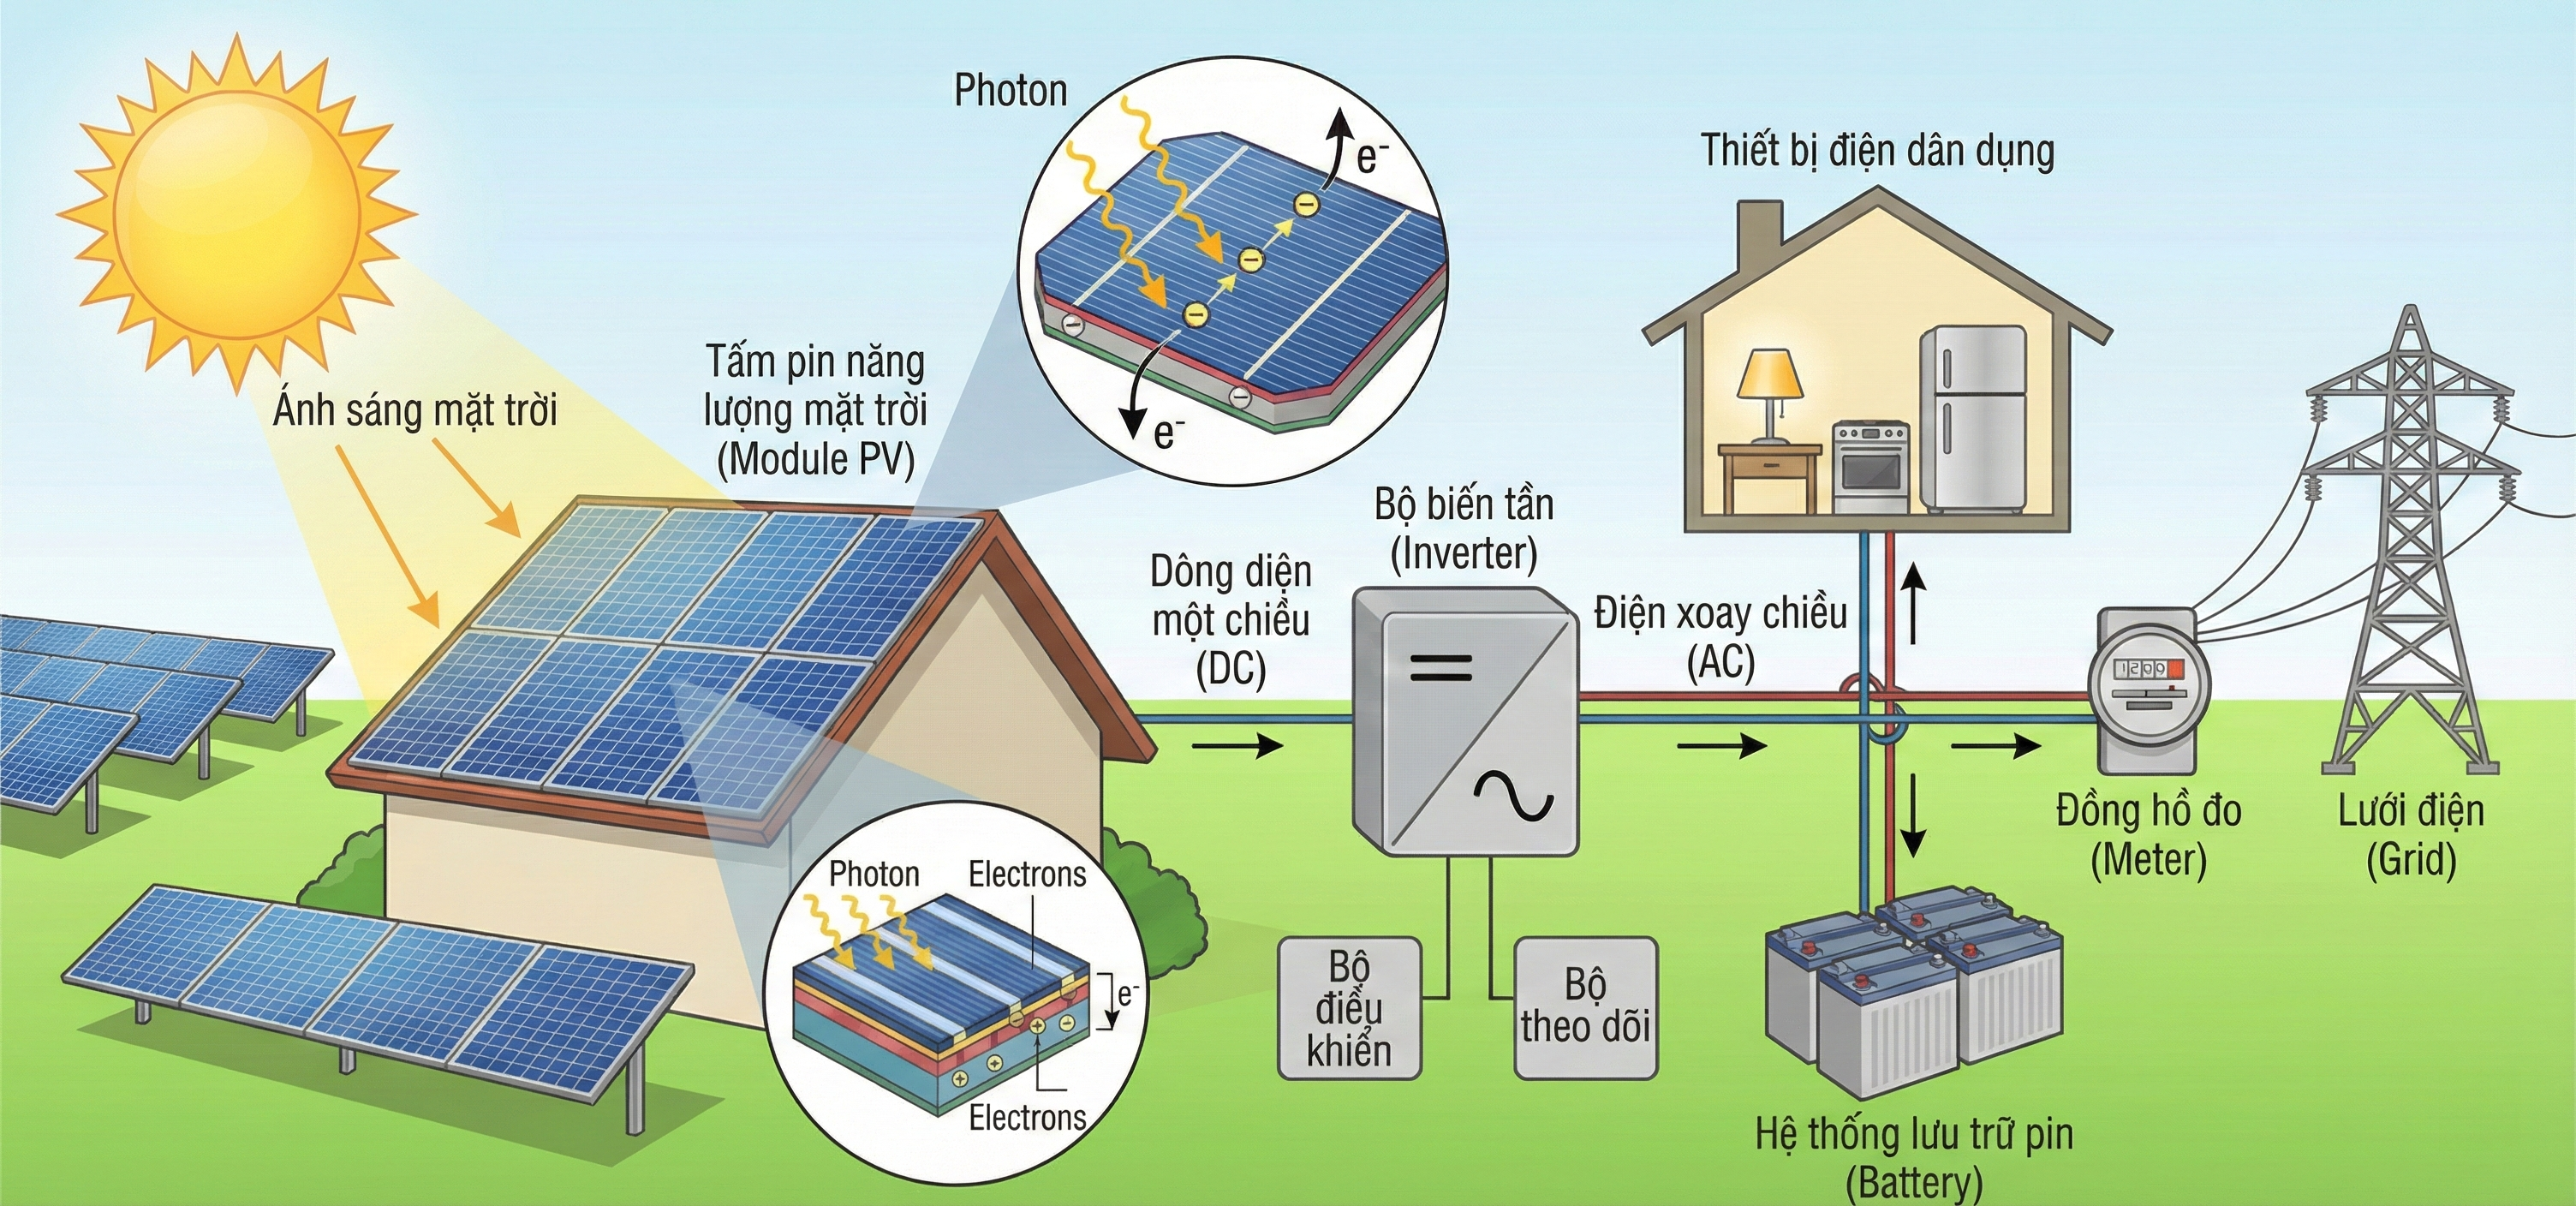
\includegraphics[width=0.8\textwidth]{images/TongQuan/pinmattroi.png}
	\end{center}
\end{frame}

%------------------------------------------------
\begin{frame}
	\frametitle{TÌNH HÌNH HỆ THỐNG PIN MẶT TRỜI TRÊN THẾ GIỚI}
	
	\vspace{0.3cm}
	
	\begin{columns}[t]
		% Cột 1: BÙNG NỔ
		\begin{column}{0.3\textwidth}
			\centering
			\includegraphics[width=0.5\textwidth]{images/TongQuan/icons/bungno.png}
			
			\vspace{0.3cm}
			
			{\Large\textbf{BÙNG NỔ}}
			
			\vspace{0.4cm}
			
			\small
			Diện mặt trời chiếm \\
			\textcolor{orange}{\textbf{73\%}} tổng công suất \\
			năng lượng tái tạo \\
			tăng thêm toàn cầu \\
			năm 2023.
		\end{column}

		\vrule width 1pt
		
		% Cột 2: CHI PHÍ
		\begin{column}{0.3\textwidth}
			\centering
			\includegraphics[width=0.5\textwidth]{images/TongQuan/icons/chiphi.png}
			
			\vspace{0.3cm}
			
			{\Large\textbf{CHI PHÍ}}
			
			\vspace{0.4cm}
			
			\small
			Chi phí lắp đặt đã giảm sâu \\
			\textcolor{orange}{\textbf{85\%}} sau một thập kỷ, trở \\
			thành nguồn năng lượng \\
			dễ tiếp cận nhất.
		\end{column}

		\vrule width 1pt
		
		% Cột 3: TIỀM NĂNG
		\begin{column}{0.3\textwidth}
			\centering
			\includegraphics[width=0.5\textwidth]{images/TongQuan/icons/tiemnang.png}
			
			\vspace{0.3cm}
			
			{\Large\textbf{TIỀM NĂNG}}
			
			\vspace{0.4cm}
			
			\small
			Việt Nam nằm trong \\
			``vùng đỏ'' bức xạ nhiệt, \\
			mang hữu tiềm năng tự \\
			nhiên lý tưởng để phát \\
			triển điện mặt trời.
		\end{column}
	\end{columns}
	
\end{frame}

\begin{frame}
\label{Bungno}
	\frametitle{TÌNH HÌNH HỆ THỐNG PIN MẶT TRỜI TRÊN THẾ GIỚI}
	\begin{center}
		\includegraphics[width=0.7\textwidth]{images/TongQuan/bieudobungno.png}
	\end{center}
\end{frame}

\begin{frame}
\label{Chiphi}
	\frametitle{TÌNH HÌNH HỆ THỐNG PIN MẶT TRỜI TRÊN THẾ GIỚI}
	\begin{center}
		\includegraphics[width=0.6\textwidth]{images/TongQuan/bieudochiphi.png}
	\end{center}
\end{frame}

\begin{frame}
\label{Nhiet}
	\frametitle{TÌNH HÌNH HỆ THỐNG PIN MẶT TRỜI TRÊN THẾ GIỚI}
	\begin{center}
		\includegraphics[width=0.8\textwidth]{images/TongQuan/bieudonhiet.png}
	\end{center}
\end{frame}

\begin{frame}
    \frametitle{TÌNH HÌNH HỆ THỐNG PIN MẶT TRỜI TRÊN VIỆT NAM}
    
    % [FIX 1] Giảm khoảng cách dưới tiêu đề (0.2 -> 0.1)
    \vspace{0.1cm} 
    
    \begin{columns}[T] 
        
        % --- CỘT TRÁI: BẢN ĐỒ ---
        \begin{column}{0.32\textwidth}
            \centering
            \vspace{0pt} 
            \includegraphics[width=0.95\textwidth]{images/TongQuan/bandonhietVietNam.png}
        \end{column}
        
        % --- CỘT PHẢI: NỘI DUNG ---
        \begin{column}{0.65\textwidth}
            \vspace{0pt} 
            
            % === PHẦN 1: PHÁP LÝ ===
            % [FIX 2] Giảm kích thước khung chứa icon (1.2cm -> 0.9cm)
            \begin{minipage}[c]{0.9cm}
                % [FIX 3] Giảm size icon (1.0cm -> 0.75cm) cho gọn
                \includegraphics[width=0.75cm]{images/TongQuan/icons/phaply.png}
            \end{minipage}%
            \hspace{0.1cm}%
            \begin{minipage}[c]{8.8cm} 
                {\Large\textbf{\textcolor{blue!70!black}{PHÁP LÝ}}}
            \end{minipage}
            
            % [FIX 4] Giảm khoảng cách dưới tiêu đề mục (0.1 -> 0.05)
            \vspace{0.05cm}
            
            \footnotesize
            \begin{itemize}
                % [FIX 5] Giảm khoảng cách giữa các item (0.1 -> 0.02)
                \setlength\itemsep{0.02cm} 
                \item Chuyển từ giai đoạn chính sách giá ưu đãi (kích cầu đầu tư ồ ạt) sang giai đoạn phát triển bền vững và có kiểm soát.
                \item Tập trung kiểm soát an toàn lưới điện và đặc biệt ưu tiên khuyến khích mô hình điện mặt trời \textbf{tự sản tự tiêu} (thay vì bán lên lưới).
            \end{itemize}
            
            % [FIX 6] Giảm khoảng cách lớn giữa 2 phần (0.4 -> 0.25)
            \vspace{0.25cm} 
            
            % === PHẦN 2: TIỀM NĂNG ===
            \begin{minipage}[c]{0.9cm}
                \includegraphics[width=0.75cm]{images/TongQuan/icons/tiemnangVietNam.png}
            \end{minipage}%
            \hspace{0.1cm}%
            \begin{minipage}[c]{8.8cm}
                {\Large\textbf{\textcolor{orange}{TIỀM NĂNG}}}
            \end{minipage}
            
            \vspace{0.05cm}
            
            \footnotesize
            \begin{itemize}
                \setlength\itemsep{0.02cm}
                \item \textbf{Việt Nam} nằm trong nhóm quốc gia có bức xạ mặt trời \textbf{tốt nhất Đông Nam Á}, đặc biệt tại miền Trung và Nam Bộ (bức xạ $>$4.6 kWh/kWp/ngày; $>$2500 giờ nắng/năm).
                \item \textbf{Miền Nam} phù hợp phát triển cả trang trại lớn và điện áp mái; \textbf{Miền Bắc} tuy bức xạ thấp hơn nhưng vẫn hiệu quả cho mô hình áp mái kết hợp lưu trữ.
            \end{itemize}
            
        \end{column}
    \end{columns}
\end{frame}

%------------------------------------------------
\section{Testing}

%------------------------------------------------
\begin{frame}
	\frametitle{Blocks}
    	\begin{block}{Block Title}
    		Block 1
    	\end{block}
    	
    	\begin{exampleblock}{Example Block Title}
    		Block 2
    	\end{exampleblock}
    	
    	\begin{alertblock}{Alert Block Title}
    		Block 3
    	\end{alertblock}
    	
    	\begin{block}{}
    		Block without a title
    	\end{block}
\end{frame}
